        %%%%%%%%%%%%%%%%%%%%%%%%%%%%%%%%%%%%%%%%%%%%%%%%%%%%%%%%%%%%%%%%%%%%%%%%%%%%%%%%%%%%
%Do not alter this block of commands.  If you're proficient at LaTeX, you may include additional packages, create macros, etc. immediately below this block of commands, but make sure to NOT alter the header, margin, and comment settings here. 
\documentclass[12pt]{article}
 \usepackage[margin=1in]{geometry} 
\usepackage{amsmath,amsthm,amssymb,amsfonts, enumitem, fancyhdr, color, hyperref,comment, graphicx, environ,mathtools, bbm, tikz, setspace, cleveref,listings, dcolumn}
\usepackage{array, multirow, caption, booktabs}
\usepackage{ mathrsfs }
\usetikzlibrary{matrix,positioning}
\tikzset{bullet/.style={circle,draw=black,inner sep=8pt}}
\DeclareMathOperator*{\argmax}{arg\,max}
\DeclareMathOperator*{\argmin}{arg\,min}
\DeclareMathOperator*{\Var}{\text{Var}}
\DeclareMathOperator*{\Cov}{\text{Cov}}

\DeclarePairedDelimiter\norm{\lVert}{\rVert}%
\newtheorem{theorem}{Theorem}
\newtheorem{lemma}[theorem]{Lemma}
\DeclareMathOperator{\eps}{\varepsilon}
\doublespacing
\DeclarePairedDelimiter\abs{\lvert}{\rvert}%
\pagestyle{fancy}
\setlength{\headheight}{65pt}
\newenvironment{problem}[2][Problem]{\begin{trivlist}
\item[\hskip \labelsep {\bfseries #1}\hskip \labelsep {\bfseries #2.}]}{\end{trivlist}}
\newenvironment{sol}
    {\emph{Solution:}
    }
    {
    \qed
    }


%%%%%%%%%%%%%%%%%%%%%%%%%%%%%%%%%%%%%%%%%%%%%%%%%%%%%%%%%%%%%%%%%%%%%%%%%%%%%%%%%


\usepackage{xcolor}
 
 


%%%%%%%%%%%%%%%%%%%%%%%%%%%%%%%%%%%%%%%%%%%%%

\rhead{Asha Bharadwaj, Caitlin Dutta, John Higgins, Alexis Smith\\Econ 899 \\ 14 September, 2022} 

%%%%%%%%%%%%%%%%%%%%%%%%%%%%%%%%%%%%%%%%%%%%%


%%%%%%%%%%%%%%%%%%%%%%%%%%%%%%%%%%%%%%

\begin{document}
\section{Solution to questions (using Julia)}
Note: I answer questions 1-3 using the output of my Julia program. I include the output for Matlab and Fortran in the next section. All code, figures, and auxiliary files can be found \href{https://github.com/johnfhiggins/F22/tree/master/Computational/PS1}{here}. 
\begin{enumerate}
	\item The agent's dynamic programming problem is as follows. Given a current level of capital $k$ and realization of productivity level $z$, the agent's value is given by the following:
	\[V(k, z) = \max_{(k', c) \in \Gamma(k,z)} u(c) + \beta \sum_{z' \in Z} V(k', z') \Pi(z', z)\]
	where $\Pi(z',z)$ is the probability of transitioning to productivity $z'$ given current state $z$, $Z = \{1.25, 0.2\}$ is the set of productivity levels, and
	\begin{align*}\Gamma(k,z) = \{(k', c) \in \mathbb{R}^2_+ \mid k' + c \leq z k^{\theta} + (1-\delta) k\}
	\end{align*}
	is the set of feasible choices of consumption and future capital given current capital $k$ and productivity $z$.
    \item Below, I plot the value function for $K$ over each state $Z$. It is evident that $V(k, z)$ is increasing in $z$ since the high productivity function lies above the low productivity function. Furthermore, it is `concave' in $K$, as the difference between the two shrinks as $K$ grows. To more clearly see these relationships, I have plotted $V(\cdot, Z^g) - V(\cdot, Z^b)$ for all $K$. It is clear that the difference is positive and decreasing in $K$, verifying the previous claims.
    \begin{center}
        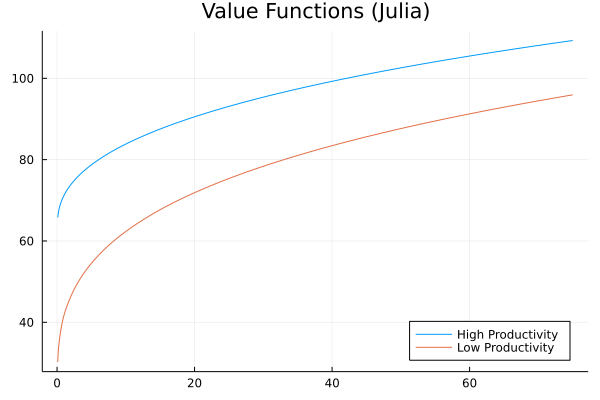
\includegraphics[scale=0.4]{vfplot.png}\\
        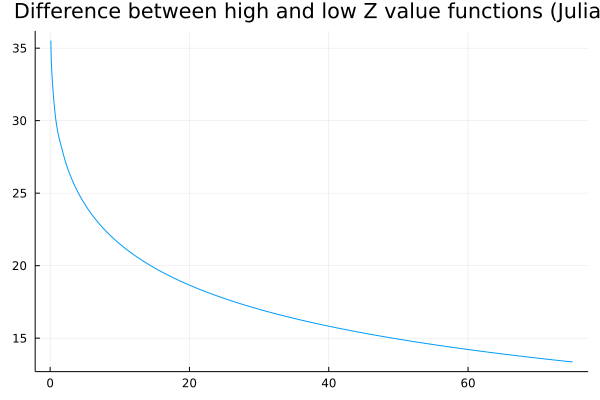
\includegraphics[scale=0.4]{netvfplot.png}\\
        Figures generated using Julia
    \end{center}
    \item The decision rule is increasing in both $K$ and $Z$. To see this, I plot the policy function as a function of $K$ for both high and low productivity levels below. For both types, $K'(k,z)$ is increasing in $k$. Furthermore, it is evident that the policy function for high productivity agents is higher than that of low productivity agents.
    \begin{center}
        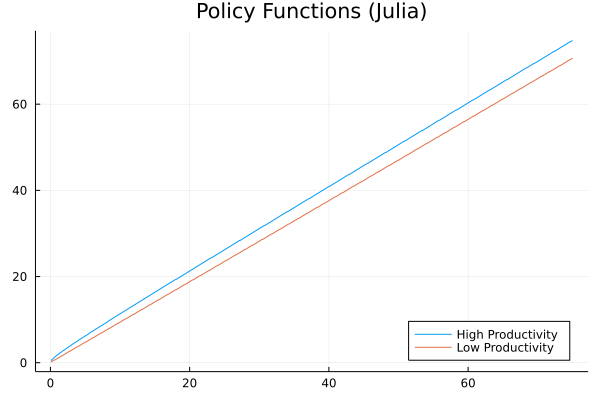
\includegraphics[scale=0.4]{pfplot.png}
    \end{center}
    However, when we plot $K'(K, Z) - K$ across $K$ in the following figure to ascertain agents' savings as a function of $K$ and $Z$, we can see that the relationship is somewhat more complicated. 
    \begin{center}
        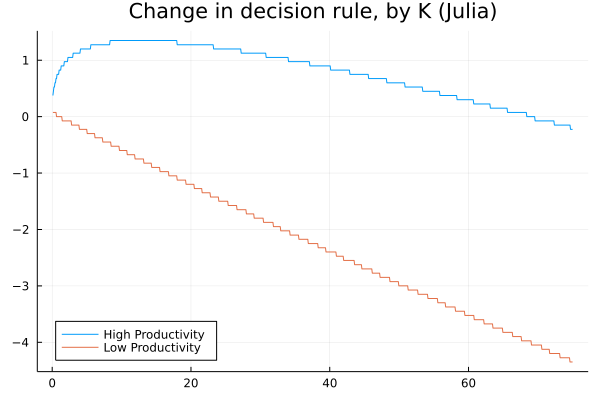
\includegraphics[scale=0.4]{netpfplot.png}
    \end{center}
    Upon inspection, we note that high productivity agents have higher savings than low productivity agents.
    
    Furthermore, low productivity agents' savings is decreasing in their current level of capital $K$.

    Finally, high productivity agents' savings are increasing in $K$ when their current level of capital is below a certain threshold (about 15 or so), and are decreasing in $K$ when their current level of capital is higher than this threshold. 

	\end{enumerate}
    
    \section{Repeating the analysis with Matlab and Fortran}
    \begin{center}
        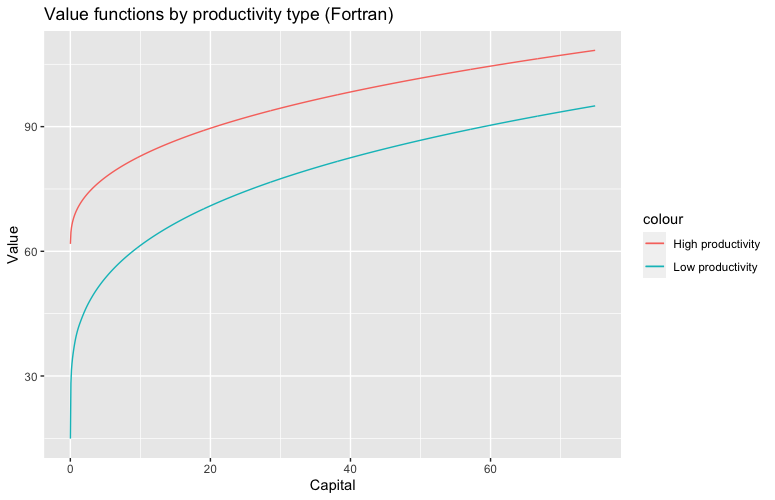
\includegraphics[scale=0.4]{for_vf.png}\\
        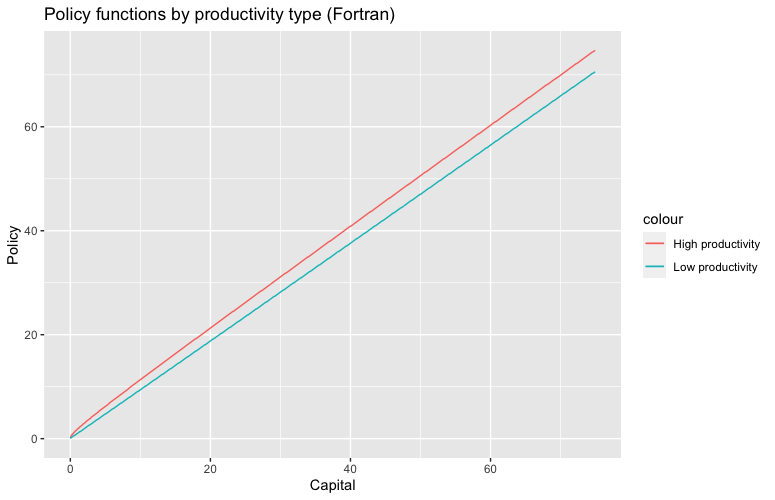
\includegraphics[scale=0.4]{for_pf.png}\\
        Results using Fortran
    \end{center}
    \begin{center}
        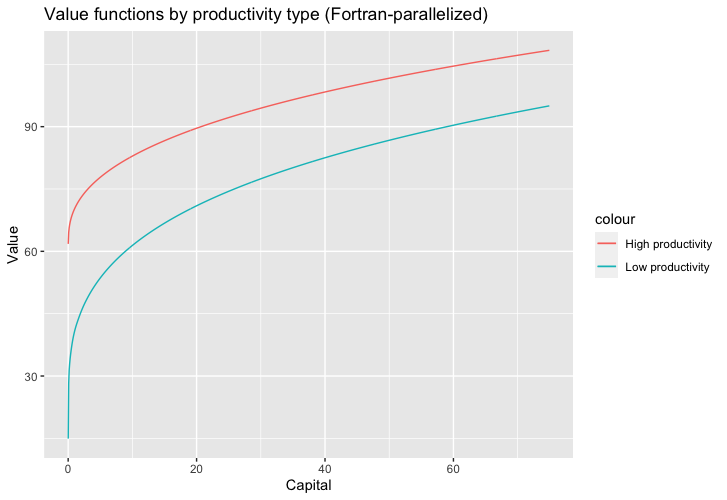
\includegraphics[scale=0.4]{for_par_vf.png}\\
        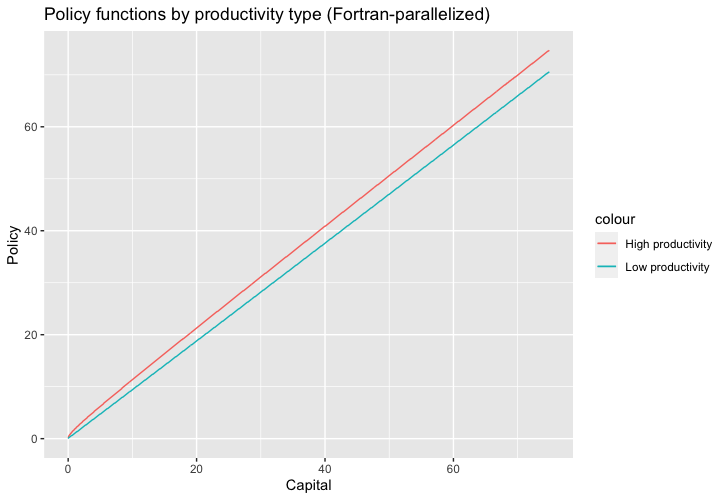
\includegraphics[scale=0.4]{for_par_pf.png}\\
        Results using Fortran (parallelized)
    \end{center}
    \begin{center}
        %insert figures here
        Results using Matlab
    \end{center}
    Time comparison:
    \begin{itemize}
        \item Julia: 3.297 seconds
        \item Julia (parallelized): 2.173 seconds
        \item Matlab: 
        \item Fortran (non-parallelized): 3.067 seconds
        \item Fortran (parallelized): 0.188 seconds
    \end{itemize}
    Note: I set the max capital level at 75 for each model. Originally, the code we were given had different capital grids (Fortran's only went up to 45, whereas the Julia one went up to 75). To enable a fair comparison, I made them all 75.
\end{document}
